%%% Document Author: J Moss
%%% Parts in LaTeX: Nicholas Dart
%%% Other Content: See authors list
%%% Document Last edit: 28.10.2014

\documentclass[11pt, article]{article}
\usepackage{a4wide}
\usepackage[english]{babel}
\usepackage{graphicx}
\usepackage{tabu}
\usepackage{textcomp}
\usepackage{fancyhdr}
\usepackage{lastpage}
\usepackage{titlesec}
\usepackage{lscape}

%%%%%%
%% Variables for version and release status
%% useage: \version
%%%%%%
\newcommand\version{Max Atkins}
\newcommand\release{CS22510 Assignment 1}
\newcommand\titleText{Assignment 1: Aphids and Ladybugs}
\newcommand\reference{CS22510 Assignment 1}

%%%%%%
%% Alias
%%%%%%
\newcommand{\sectionbreak}{\clearpage} 	%% Allways start a section on a new page

\title{ \huge CS22510  C++, C and Java Programming Paradigms\\ \Large \titleText}
\author{
	\vspace{100pt}
	\begin{tabular}{ r || l }
		Author 	& Max Atkins \\
						& \\
		Date Published  & \today \\
						&\\
		Department		& Computer Science \\
						&\\
		Address			& Aberystwyth University \\
						& Penglais Campas \\
						& Ceredigion \\
						& SY23 3DB \\
	\end{tabular} \\
	Copyright \textcopyright Aberystwyth University 2015
	%get rid of the date on the titlepage
	\date{}
}

\pagestyle{fancy}
\fancyhf{}
\rhead{\version}
\lhead{\release}
\rfoot{Page \thepage \hspace{1pt} of \pageref{LastPage}}
\lfoot{Aberystwyth University - Computer Science}

\begin{document}
	\setcounter{page}{1}

	\maketitle

	\tableofcontents

	\section{Introduction}
		%%\input{foo/bar.tex}

Aphids and Ladybugs was my first opportunity to properly work with C++, after working with many languages such as Java, C, HTML, JavaScript, Php etc. This language has been, by far, the most different and complex language I've had to learn since I started. I have thoroughly enjoyed the challenge this has proved to me, and my skills have vastly improved, both in C++ and in design patterns. 

This assignment required me to design an Object-Oriented (OO) simulation of aphids and ladybugs living together in a 2D world, where they fight and re-produce, attempting to live for as long as possible. Being required to take an OO approach has forced me to fully embrace the language of C++: it's features, it's flexibility and it's complexity. 

	\section{Design}
		%%\input{foo/bar.tex}

My design involves a Manager class which controls everything in the program: creation of animals, calling relevant functions on each animal and the grid, passing correct collections of animals for the grid to draw etc. The Manager class is the core of the program, linking all parts of it together into a fluid program. I have a Grid class which is created by Manager, it implements functions to draw the grid, changing based on the vectors it receives. I have an Animal superclass, of which, Aphid and Ladybug inherit common characteristics (functions and variables), and then the subclasses implement their own unique characteristics, for example, a ladybug moves in a preferred direction whereas an Aphid moves in random directions. The Animal superclass inherits a Visitor pattern definition class. 

	\begin{figure}[ht!]
	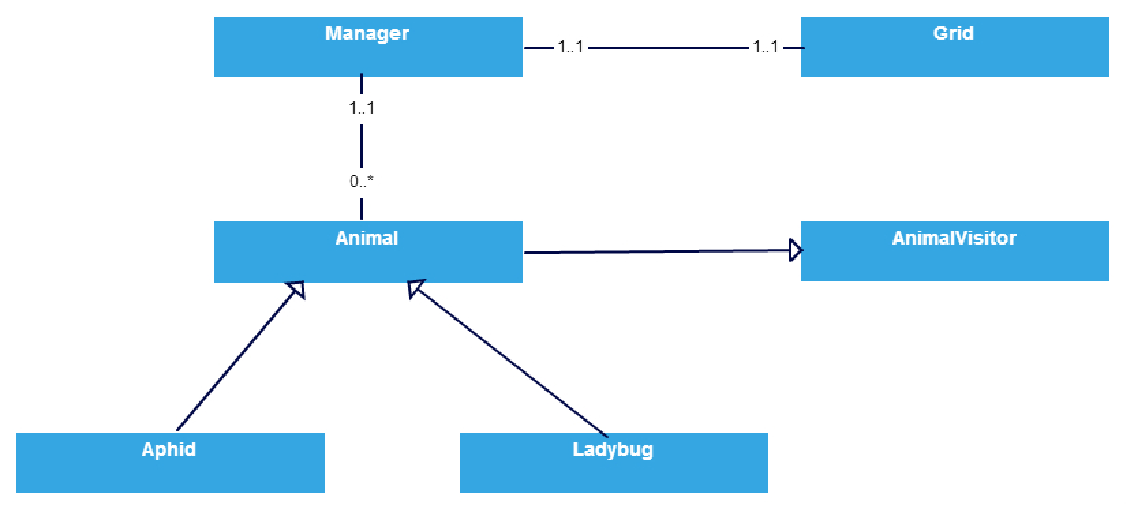
\includegraphics[]{ClassDiagram.pdf}
 	\caption{Class Diagram}
	\end{figure}
	
	\subsection{Manager Design}
	
	The core class of my project is the Manager. This class creates instances of all the other classes when necessary, and calls all the implemented functions of those classes to make the program run. The Manager has functions such as  setVectors() which keeps track of aphids, ladybugs and updates the vector of allAnimals to hold them all. This allAnimals vector holds pointers to Animals to allow the actual objects to be deleted. The Manager's core function is updateAll(), which calls relevant functions on it's Animal objects to pass to the Grid object for displaying the grid. This Manager class is a good example of OO implementation, as it reflects a real-world situation, where certain objects have no idea of others and only have to worry about themselves. It is an extensible design that allows more animals to be implemented easily.   
	
	\subsection{Grid Design}
	
	The Grid class is very simple, and not very OO. It takes vectors of aphids and ladybugs, and loops through them checking their positions on the grid and prints out a letter and a count for each object on the grid. This is done through various loops and if statements, rather than effective OO programming and is a major point of improvement.
	
	\subsection{Animal Design}
	
	For designing my animals, I use a Superclass parent (Animal) which holds common characteristics which are shared across all animals, such as set and getPosition(), set and getLife() etc. It provides functions that are overridden by it's children, update() so that they can implement their own update behaviour. Each animal also implements their own functions, such as Ladybug::changePreferredDirection() and Aphid::setGroupKillProb(). Polymorphism is handled in such a way that any animal can be passed to almost any function, and the correct implementations will be chosen. More on this in 2.4. 
	
	\subsection{Visitor Design Pattern}
	
	To allow ladybugs and aphids to interact with each other polymorphically, without the need for many if statements, loops and unnecessary typeid()s or dynamiccasts, I have implemented the Visitor Design Pattern. By creating another Superclass AnimalVisitor, which is a parent of Animal, it allows me to create visit() functions that take an Animal reference and choose the correct implementation based on the animal type that called it and the animal type passed to it. For example, if a Ladybug called visitWith(Aphid), then the Ladybug would call the implementation for attacking the aphid. If an Aphid called visitWith(Aphid), then the implementation for reproduction is called. This is a very efficient and very strong OO design pattern that allows me to use one function polymorphically for every Animal type combination possible. 
	
	\section{Issues and Improvements}
		%%\input{foo/bar.tex}
	
	My program is not without flaw, by far. If I was to do this assignment again, with more time, I would implement a better Grid class. I would create a Cell class which can contain information about it's neighbours, which animals it is holding and any other implementable functionality. This would greatly increase the effectiveness and efficiency of my program. 
	
	I would create more OO implementations to reduce the amount of if statements I have in my code for specific Animal types, so that more animal types can be implemented with less effort. 
	
	There is a bug in my system at the moment, where, upon reaching ~10,000-15,000 objects, a segmentation fault occurs when calling getReproduce() on an Animal. I have spent many hours attempting to find the cause of this, but it seems to be such an unusual bug that I can not work it out. I don't understand how a program can do the same thing 15,000 times, and then fail. 

	\section{Self-Evaluation}
		%%\input{foo/bar.tex}
	
	At the start of this assignment, my knowledge of C++ was very limited, and my knowledge of OO was only slight better. Had I had a better understanding of OO, I would have created a much stronger architecture from the start, before getting to a point where I realise I could have done something better. For example, having created the Grid object early in the assignment period, I built upon it until it was very difficult to change. 
	
	My knowledge and experience in both of these areas, however, have vastly improved upon completing this assignment. I have thoroughly enjoyed the interesting and entertaining context, and have fallen in love with C++. I look forward to my next C++ challenge. 


	%%\begin{landscape}

		%%\section{Bar}
			%%\input{far/foo.tex}

	%%\end{landscape}


\end{document}